\documentclass[xcolor={dvipsnames}]{beamer}

\usepackage{lmodern}
\usepackage[utf8]{inputenc}
\usepackage{amssymb, amsmath, amsthm, graphicx}
\usepackage[super]{nth}
\usepackage{tikz}

\usetheme{Frankfurt}
\renewcommand{\phi}{\varphi}
\renewcommand{\epsilon}{\varepsilon}
\newcommand{\df}[1]{\textcolor{BrickRed}{\emph{#1}}}
\renewcommand{\th}[1]{\textcolor{Fuchsia}{\emph{#1}}}
\renewcommand{\hat}{\widehat}

\newcommand{\cD}{\mathcal{D}}
\newcommand{\cL}{\mathcal{L}}
\newcommand{\cM}{\mathcal{M}}
\newcommand{\cN}{\mathcal{N}}
\newcommand{\cX}{\mathcal{X}}
\newcommand{\cZ}{\mathcal{Z}}
\newcommand{\EE}{\mathbb{E}}
\newcommand{\vv}{\mathbf{v}}
\newcommand{\vw}{\mathbf{w}}
\newcommand{\vx}{\mathbf{x}}
\newcommand{\vy}{\mathbf{y}}
\newcommand{\vY}{\mathbf{Y}}
\newcommand{\One}{\mathbf{1}}
\newcommand{\vbeta}{\boldsymbol{\beta}}


\newcommand{\RR}{\mathbb{R}}

\newcommand{\train}{{\text{train}}}
\newcommand{\test}{{\text{test}}}

\DeclareMathOperator*{\argmin}{argmin}
\DeclareMathOperator{\Bias}{Bias}
\DeclareMathOperator{\Var}{Var}
\DeclareMathOperator{\MSE}{MSE}
\DeclareMathOperator{\MISE}{MISE}
\DeclareMathOperator{\Bernoulli}{Bernoulli}

\title[DATA 607]{DATA 607 Statistical and Machine Learning\\
\textit{Session 2: Linear Smoothers}}
\author{Matthew Greenberg}
\institute[]{Department of Mathematics and Statistics\\
University of Calgary}
\date{28.02.2020}



% \includeonlyframes{current}

\begin{document}

\frame{\titlepage}

\begin{frame}{This Evening's Agenda}
        \setlength\parskip{0.75em}

    \tableofcontents
    
\end{frame}



\section{Regressors/Smoothers}
\begin{frame}{Regressors/Smoothers}
    \setlength\parskip{0.5em}
    \textbf{Regression Models} or \textbf{Regressors} are models for fitting curves to data.

    \textbf{Smoother} is a synonym for regressor, typically used in the context of nonparametric models.
    \begin{center}
        \includegraphics[scale=0.6]{smoother.pdf}
    \end{center}
\end{frame}

\section{Linear Smoothers}
\subsection{Definition}
\begin{frame}{Linear Smoothers}
    \setlength\parskip{0.5em}
    \textbf{Dataset:}
    \[
        (\vx_1, Y_1),\ldots,(\vx_n, Y_n)
    \]
    
    \textbf{Regression Model:}
    \[
        Y_i = r(\vx_i) + \epsilon_i
    \]

    \begin{block}{Definition}
    A \emph{linear smoother} is an estimator of $r$ of the form
    \[
        \hat r(\vx) = \sum_{i=1}^n w_i(\vx)Y_i = \vw(\vx)\cdot \vY.
    \]
    \end{block}

    The $w_i(\vx)$ are called \emph{weights}.

    Linear smoother are so named because they are \emph{linear functions of $\vY$}.
    Their graphs need not be lines!
\end{frame}

\subsection{Example: Linear Regression}
\begin{frame}{Example 1: Linear Regression}
    \setlength\parskip{1em}
    \textbf{Dataset:}
    \[
        (\vx_1, Y_1),\ldots,(\vx_n, Y_n),\qquad \vx_i\in\RR^{1\times p},\qquad Y_i\in\RR
    \]

    \textbf{Regression Model:}
    \begin{align*}
        Y_i &= \beta_0 + \beta_1x_{i,1}+\cdots + \beta_p x_{i,p} + \epsilon\\[1ex]
            &= \underbrace{\begin{pmatrix}1&\vx_i\end{pmatrix}}_{1\times(p+1)}\vbeta + \epsilon,
    \end{align*}
    where
    \[
        \vbeta = \begin{pmatrix}
            \beta_0\\\vdots\\\beta_p
        \end{pmatrix}\in\RR^{(p+1)\times 1}.
    \]
\end{frame}

\begin{frame}

    \textbf{Least-Squares Line:}
    \[
        \hat r(\vx) = \begin{pmatrix}
            1&\vx
        \end{pmatrix}\hat{\vbeta},\tag{$*$}
    \]
    $\hat\vbeta$ is the least-squares solution of
    \[
        X\vbeta = \vY,\qquad\text{where}\qquad X = \begin{pmatrix}
            1&\vx_1\\\vdots&\vdots\\1&\vx_n
        \end{pmatrix}\in\RR^{n\times(p+1)}.
    \]
    Explicitly,
    \[
        \hat\vbeta = (X^TX)^{-1}X^T\vY.
    \]
    Substituting into $(*)$,
    \[
        \hat r(\vx) = \underbrace{(\vx(X^TX)^{-1}X^T)}_{\vw(\vx)}\vY.
    \]

    Thus, $\hat r$ is a linear smoother.
\end{frame}

% \begin{frame}
%     \frametitle{Coding Activity 1}
%     \begin{enumerate}
%         \setlength\parskip{0.5em}
%         \item Mock some data, \[
%             (x_0, y_0),\;\ldots,\;(x_{19}, y_{19}),\qquad x_i\in(0,1),\; y_i\in\RR,
%         \]
%         suitable for linear regression:
%                 \begin{enumerate}
%                     \setlength\parskip{0.5em}
%                     \item Choose $\vbeta_0$ and $\beta_1$ uniformly at random from the intervals $(0,1)$ the and $(-1, 0)$, respectively.
%                     \item Choose $x_0,\ldots,x_{19}$ uniformly at random from the interval $(-1, 1)$.
%                     \item Draw a random sample $\epsilon_0,\ldots,\epsilon_{19}$ from $N(0,0.2)$.
%                     \item Set $y_i = \beta_0 + \beta_1 x_i + \epsilon_i$.
%                 \end{enumerate}
%             \item Plot $y$ versus $x$. It should look roughly linear.
%             \item Write a function that computes $\vw(x)$ from $x$.
%             \item Plot the graph of $y=\hat r(x)$.
%     \end{enumerate}
%     \end{frame}
    
\subsection{Example: $k$-Nearest Neighbors}
\begin{frame}{Example 2: $k$-Nearest Neightbor Smoother}
    \setlength\parskip{1em}

    \textbf{Data:} $$(\vx_0,Y_0)\;\ldots,\;(\vx_{n-1}, Y_{n-1})$$
    
    \textbf{Regression Model:}
    \[
        Y_i = r(\vx_i) + \epsilon_i
    \]

    \textbf{$k$-Nearest Neighbors:} 
    \[
        N_k(\vx) = \text{the $k$ elements of $\vx_0,\;\ldots,\;\vx_{n-1}$ closest to $\vx$}
    \]

    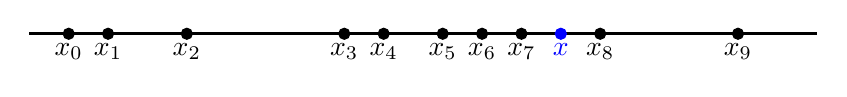
\begin{tikzpicture}
        \draw[very thick] (0, 0) -- (10,0);
        \filldraw[black] (0.5,0) circle (2pt) node[below] {$x_0$};
        \filldraw[black] (1,0) circle (2pt) node[below] {$x_1$};
        \filldraw[black] (2,0) circle (2pt) node[below] {$x_2$};
        \filldraw[black] (4,0) circle (2pt) node[below] {$x_3$};
        \filldraw[black] (4.5,0) circle (2pt) node[below] {$x_4$};
        \filldraw[black] (5.25,0) circle (2pt) node[below] {$x_5$};
        \filldraw[black] (5.75,0) circle (2pt) node[below] {$x_6$};
        \filldraw[black] (6.25,0) circle (2pt) node[below] {$x_7$};
        \filldraw[blue] (6.75,0) circle (2pt) node[below] {$x$};
        \filldraw[black] (7.25,0) circle (2pt) node[below] {$x_8$};
        \filldraw[black] (9,0) circle (2pt) node[below] {$x_9$};
        % \draw (5, 0.5) rectangle (8.5, -0.5);
    \end{tikzpicture}
    \[
        N_3(x) = \{x_6, x_7, x_8\}
    \]
\end{frame}

\begin{frame}
    \setlength\parskip{1em}

    \begin{block}{Definition}
    The \textbf{$k$-nearest neighbor smoother} is the estimator of $r$ is defined by
    \begin{align*}
        \hat r_k(\vx) 
        &= \text{average of the $Y_i$ for which $\vx_i\in N_k(\vx)$}\\[2ex]
        &= \sum_{i=0}^{n-1} w_i(\vx)Y_i,\quad\text{where}\quad
        w_i(\vx)=\begin{cases}
            \dfrac1k&\text{if $\vx_i\in N_k(\vx)$,}\\[2ex]
            0&\text{otherwise.}
        \end{cases}
    \end{align*}
    \end{block}

    \bigskip
    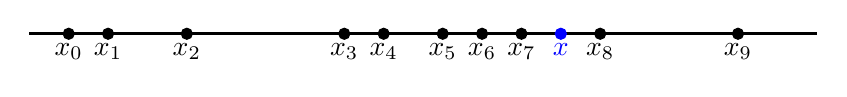
\begin{tikzpicture}
        \draw[very thick] (0, 0) -- (10,0);
        \filldraw[black] (0.5,0) circle (2pt) node[below] {$x_0$};
        \filldraw[black] (1,0) circle (2pt) node[below] {$x_1$};
        \filldraw[black] (2,0) circle (2pt) node[below] {$x_2$};
        \filldraw[black] (4,0) circle (2pt) node[below] {$x_3$};
        \filldraw[black] (4.5,0) circle (2pt) node[below] {$x_4$};
        \filldraw[black] (5.25,0) circle (2pt) node[below] {$x_5$};
        \filldraw[black] (5.75,0) circle (2pt) node[below] {$x_6$};
        \filldraw[black] (6.25,0) circle (2pt) node[below] {$x_7$};
        \filldraw[blue] (6.75,0) circle (2pt) node[below] {$x$};
        \filldraw[black] (7.25,0) circle (2pt) node[below] {$x_8$};
        \filldraw[black] (9,0) circle (2pt) node[below] {$x_9$};
    \end{tikzpicture}
    \[
        N_3(x) = \{x_6, x_7, x_8\},\qquad \hat r_3(x) = \frac13(Y_6 + Y_7 + Y_8)
    \]
\end{frame}

\begin{frame}
    \setlength\parskip{1em}
    \textbf{$3$-Nearest Neighbors:} 

    \bigskip
    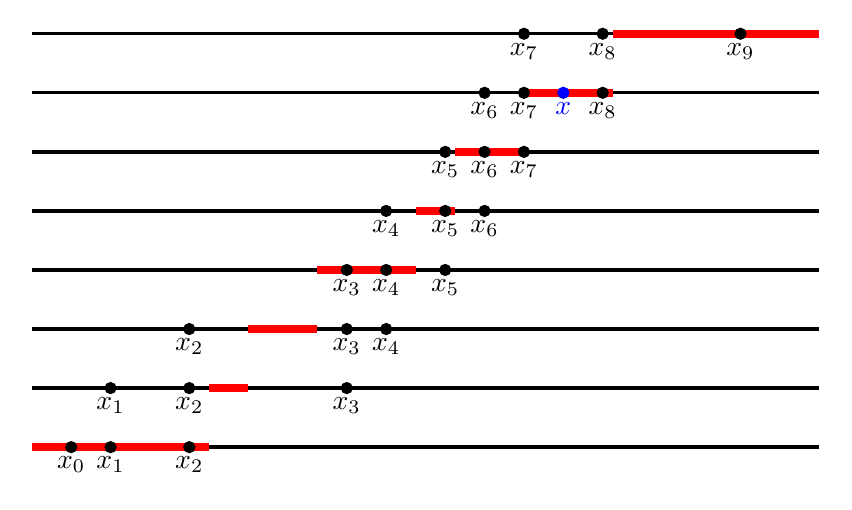
\begin{tikzpicture}
        \draw[very thick] (0, 0) -- (10,0);
        \draw[red, line width=3pt] (0,0) -- (2.25, 0);
        
        \draw[very thick] (0, 0.75) -- (10,0.75);
        \draw[red, line width=3pt] (2.25,0.75) -- (2.75, 0.75);

        \draw[very thick] (0, 1.5) -- (10,1.5);
        \draw[red, line width=3pt] (2.75, 1.5) -- (3.625, 1.5);

        \draw[very thick] (0, 2.25) -- (10,2.25);
        \draw[red, line width=3pt] (3.625, 2.25) -- (4.875, 2.25);

        \draw[very thick] (0, 3) -- (10,3);
        \draw[red, line width=3pt] (4.875, 3) -- (5.375, 3);

        \draw[very thick] (0, 3.75) -- (10,3.75);
        \draw[red, line width=3pt] (5.375, 3.75) -- (6.25, 3.75);

        \draw[very thick] (0, 4.5) -- (10,4.5);
        \draw[red, line width=3pt] (6.25, 4.5) -- (7.375, 4.5);

        \draw[very thick] (0, 5.25) -- (10,5.25);
        \draw[red, line width=3pt] (7.376, 5.25) -- (10, 5.25);

        \filldraw[black] (0.5,0) circle (2pt) node[below] {$x_0$};
        \filldraw[black] (1,0) circle (2pt) node[below] {$x_1$};
        \filldraw[black] (2,0) circle (2pt) node[below] {$x_2$};
        
        \filldraw[black] (1,0.75) circle (2pt) node[below] {$x_1$};
        \filldraw[black] (2,0.75) circle (2pt) node[below] {$x_2$};
        \filldraw[black] (4,0.75) circle (2pt) node[below] {$x_3$};
        
        \filldraw[black] (2,1.5) circle (2pt) node[below] {$x_2$};
        \filldraw[black] (4,1.5) circle (2pt) node[below] {$x_3$};
        \filldraw[black] (4.5,1.5) circle (2pt) node[below] {$x_4$};
        
        \filldraw[black] (4,2.25) circle (2pt) node[below] {$x_3$};
        \filldraw[black] (4.5,2.25) circle (2pt) node[below] {$x_4$};
        \filldraw[black] (5.25,2.25) circle (2pt) node[below] {$x_5$};
        
        \filldraw[black] (4.5,3) circle (2pt) node[below] {$x_4$};
        \filldraw[black] (5.25,3) circle (2pt) node[below] {$x_5$};
        \filldraw[black] (5.75,3) circle (2pt) node[below] {$x_6$};
        
        \filldraw[black] (5.25,3.75) circle (2pt) node[below] {$x_5$};
        \filldraw[black] (5.75,3.75) circle (2pt) node[below] {$x_6$};
        \filldraw[black] (6.25,3.75) circle (2pt) node[below] {$x_7$};
        
        \filldraw[black] (5.75,4.5) circle (2pt) node[below] {$x_6$};
        \filldraw[black] (6.25,4.5) circle (2pt) node[below] {$x_7$};
        \filldraw[black] (7.25,4.5) circle (2pt) node[below] {$x_8$};
        \filldraw[blue] (6.75,4.5) circle (2pt) node[below] {$x$};
        
        \filldraw[black] (6.25,5.25) circle (2pt) node[below] {$x_7$};
        \filldraw[black] (7.25,5.25) circle (2pt) node[below] {$x_8$};
        \filldraw[black] (9,5.25) circle (2pt) node[below] {$x_9$};
    \end{tikzpicture}
\end{frame}


\begin{frame}{Sample Plots}
    \includegraphics[scale=0.32]{knn_four_plots_1.pdf}
\end{frame}

\begin{frame}
    \includegraphics[scale=0.32]{knn_four_plots_2.pdf}
\end{frame}

\begin{frame}{Overfitting and Underfitting}
    \setlength\parskip{1em}
    \includegraphics[scale=0.32]{knn_two_plots.pdf}

    For small $k$, the graphs of $\hat r(x)$ are too wiggly,
    fitting the noisy sample \emph{too closely}.
    We've \textbf{overfit} (\textbf{undersmoothed}) the data.


    For big $k$, the graphs of $\hat{r}(x)$ don't fit data very well (they're too flat).
    We've \textbf{underfit} (\textbf{oversmoothed}) the data.

    Is there a ``right'' $k$?
\end{frame}

\subsection{Example: Sliding Window}
\begin{frame}{Example 3: The Sliding Window Smoother}
    \setlength\parskip{0.75em}

    \textbf{Data:} $$(\vx_0,Y_0)\;\ldots,\;(\vx_{n-1}, Y_{n-1})$$
    
    \textbf{Regression Model:}
    \[
        Y_i = r(\vx_i) + \epsilon_i
    \]

    \textbf{$h$-neighbors:} 
    \begin{align*}
        N_h(\vx) &= \text{the elements of $\vx_0,\;\ldots,\;\vx_{n-1}$ within a distance $h$ of $\vx$}\\[1ex]
        &= \{\vx_i : \|\vx_i - \vx\| < h\}
    \end{align*}

\end{frame}
        

\begin{frame}
    \setlength\parskip{0.75em}

\begin{block}{Definition}
    The \textbf{sliding window smoother with bandwidth $h>0$} is the estimator of $r$ defined by
    \begin{align*}
        \hat r_h(\vx) 
        &= \text{average of the $Y_i$ for which $\|\vx - \vx_i\|<h$}\\[1ex]
        % &= \frac{\sum_{\|\vx_i - \vx\|< h}Y_i}{\sum_{\|\vx_i - \vx\|< h}1}\\
        &= \sum_{i=0}^{n-1} w_i(\vx)Y_i,\quad\text{where}\quad
        w_i(\vx)=\begin{cases}
            \dfrac1{\#N_h(\vx)}&\text{if $\vx_i\in N_h(\vx)$,}\\[2ex]
            0&\text{otherwise.}
        \end{cases}
    \end{align*}
\end{block}

\bigskip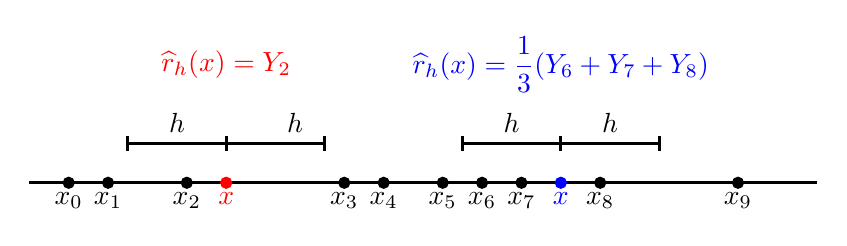
\begin{tikzpicture}
    \draw[very thick] (0, 0) -- (10,0);
    \filldraw[black] (0.5,0) circle (2pt) node[below] {$x_0$};
    \filldraw[black] (1,0) circle (2pt) node[below] {$x_1$};
    \filldraw[black] (2,0) circle (2pt) node[below] {$x_2$};
    \filldraw[red] (2.5,0) circle (2pt) node[below] {$x$};
    \draw[very thick] (1.25, 0.5) -- (1.875, 0.5) node[above] {$h$} -- (3.375, 0.5) node[above] {$h$} --  (3.75, 0.5);
    \draw[very thick] (1.25, 0.6) -- (1.25, 0.4);
    \draw[very thick] (2.5, 0.6) -- (2.5, 0.4);
    \draw[very thick] (3.75, 0.6) -- (3.75, 0.4);
    \filldraw[black] (4,0) circle (2pt) node[below] {$x_3$};
    \filldraw[black] (4.5,0) circle (2pt) node[below] {$x_4$};
    \filldraw[black] (5.25,0) circle (2pt) node[below] {$x_5$};
    \filldraw[black] (5.75,0) circle (2pt) node[below] {$x_6$};
    \filldraw[black] (6.25,0) circle (2pt) node[below] {$x_7$};
    \filldraw[blue] (6.75,0) circle (2pt) node[below] {$x$};
    \draw[very thick] (5.5, 0.5) -- (6.125, 0.5) node[above] {$h$} -- (7.375, 0.5) node[above] {$h$} --  (8, 0.5);
    \draw[very thick] (5.5, 0.6) -- (5.5, 0.4);
    \draw[very thick] (6.75, 0.6) -- (6.75, 0.4);
    \draw[very thick] (8, 0.6) -- (8, 0.4);
    \filldraw[black] (7.25,0) circle (2pt) node[below] {$x_8$};
    \filldraw[black] (9,0) circle (2pt) node[below] {$x_9$};

    \node[red] at (2.5, 1.5) {$\hat r_h(x) = Y_2$};
    \node[blue] at (6.75, 1.5) {$\hat r_h(x) = \dfrac13(Y_6+Y_7+Y_8)$};
\end{tikzpicture}
\end{frame}

\begin{frame}{Sample Plots}%{\textsc{$k$-nearest neighbors}}
    \includegraphics[scale=0.32]{la_four_plots_1.pdf}
\end{frame}

\begin{frame}{}%{\textsc{$k$-nearest neighbors}}
    \includegraphics[scale=0.32]{la_four_plots_2.pdf}
\end{frame}

\begin{frame}{Overfitting and Underfitting}
    \setlength\parskip{1em}
    \includegraphics[scale=0.32]{sliding_window_two_plots.pdf}

    For small $h$, the graphs of $\hat r(x)$ are too wiggly,
    fitting the noisy sample \emph{too closely}.
    We've \textbf{overfit} (\textbf{undersmoothed}) the data.


    For large $h$, the graphs of $\hat{r}(x)$ don't fit data very well (they're too flat).
    We've \textbf{underfit} (\textbf{oversmoothed}) the data.

    Is there a ``right'' $h$?
\end{frame}



\section{Evaluating Smoothers and Tuning Parameters}

\subsection{Prediction Error}
\begin{frame}
    \frametitle{Prediction Error}
    \setlength\parskip{0.75em}

    We evaluate a regressor based on the accuracy of its predictions.

    Let $\hat r_\cD$ be a regressor trained on the data set $\cD$.

    Assume we are in possession of a \textbf{test set},
    $$\cD_\test=\{(\vx_1,Y_1),\;\ldots,\;(\vx_n, Y_n)\},$$
    i.e., a random sample drawn from the \textbf{same distribution} as --- but \textbf{independently} of --- $\cD$.

    The \textbf{expected prediction error} of $\hat r_\cD$ is approximately the average error on $\cD_\test$:
    \[
        \text{test error} = \frac1n\sum_{i=1}^n (Y_i - \hat r_\cD(\vx_i))^2
    \]
\end{frame}

\subsection{Train/Test Split}
\begin{frame}
    \frametitle{Train/Test Split}
    \setlength\parskip{1em}

    \textbf{Split} you data set $\cD$ into two disjoint subsets: A larger \textbf{training set}, $\cD_\train$, and a smaller \textbf{testing set}, $\cD_\test$.

    Train your model on $\cD_\train$, the use $\cD_\test$ to estimate its prediction error.

    Training error typically \textbf{underestimates} prediction error!
\end{frame}


\begin{frame}
    \frametitle{Tuning Model Parameters Using a Test Set}
    \setlength\parskip{1em}

    Given a test set, $$\cD_\test = \{(\vx_1,Y_1),\;\ldots,\;(\vx_n, Y_n)\},$$
    choose your parameters
    ($k$ for $k$-nearest neighbors, $h$ for sliding window)
    to \textbf{minimize}
    
    \[
        \text{test error} = \frac1n\sum_{i=1}^n (Y_i - \hat r(\vx_i))^2,
    \]
    our proxy for the expected prediction error.

    Compute the test error for a range of values of $k$ or $h$,
    and choose the parameter value giving the smallest test error.
\end{frame}

\subsection{Cross-Validation}
\begin{frame}{$K$-Fold Cross Validation}
    \setlength\parskip{0.75em}
    \textbf{Data set:}
    $$\cD = \{(\vx_1,Y_1),\;\ldots,\;(\vx_n, Y_n)\},$$

    When $n$ is small, it may be undesirable to set aside a test set for tuning parameters.
    \textbf{Cross-validation} offers an alternative.

    Partition $\{1,\ldots,n\}$ into $K$ \textbf{folds}, $I_1,\ldots,I_K$, of roughly equal size:
    \[
        \cD = I_1\cup I_2\cup\cdots\cup I_K,\qquad \#I_j\approx \frac nK
    \]
    We get $K$ train/test splits:
    \begin{align*}
        \text{training set}& =\cD_h^{-j} = \{(\vx_i, Y_i) : i\notin I_j\},&&\text{size }\frac{K-1}Kn\\
        \text{testing set}& = \cD_h^{j}  = \{(\vx_i, Y_i) : i\in I_j\}&&\text{size }\frac{1}Kn
    \end{align*}
\end{frame}

\begin{frame}
    \setlength\parskip{0.75em}
    Compute $\hat r_h^{-j}$ by training your model on $\cD_h^{-j}$.

    Estimate the prediction error of $\hat r_h^{-j}$ on the test set $\cD_h^{j}$:
    \[
        E_{h,j} = \text{error on $\cD_h^{j}$} = \sum_{i\in I_j}\big(Y_i - \hat r_h^{-j}(\vx_i)\big)^2
    \]

    Compute the weighted average of these $K$ measurements,
    giving an overall error measurement for the parameter value, $h$:
    
    \begin{block}{Definition}
        The \textbf{$K$-Fold Cross Validation Score} is
        \[
           E_h = \sum_{j=1}^K\frac{\# I_j}{n}\sum_{i\in I_j}\big(Y_i - r_h^{(-I_j)}(x_i)\big)^2.
        \]
    \end{block}
    
    In practice, $K$ is usually $5$ (\texttt{sklearn}'s default) or $10$ or $n$.
\end{frame}

\begin{frame}
    \frametitle{Leave-One-Out Cross-Validation (LOOCV)}
    \setlength\parskip{0.75em}

    \textbf{Leave-One-Out Cross-Validation} is another name for $n$-fold cross-validation.

    In this case, the folds and testing sets are singletons,
    \[
        I_1=\{1\},\;\ldots,\; I_n=\{n\}
    \]
    \[
        \cD_h^1=\{(\vx_1,Y_1)\},\;\ldots,\; \cD_h^n=\{(\vx_n,Y_n)\},
    \]
    while the training sets, $\cD_h^{-j}$, have size $n-1$.

    \begin{block}{Definition}
        The \textbf{Leave-One-Out Cross Validation Score} is
        \[
           E_h = \frac1n\sum_{j=1}^n\sum_{i\neq j}\big(Y_i - r_h^{(-j)}(\vx_i)\big)^2.
        \]
    \end{block}

\end{frame}

% \begin{frame}{\textsc{Coding activity 2}}
%     \emph{But}, we can work in an artificial situation where we \emph{do} know $r(x)$:


%     \begin{itemize}\setlength{\itemsep}{1ex}
%         \item Choose:
%         \begin{itemize}
%             \item a function, $r(x)$
%             \item $x_1,\ldots,x_n$
%             \item a fine partition, $P$, of an interval containing the $x_i$
%             \item $k$ (or $h$)
%         \end{itemize}
%             \item for $k=1,\ldots,K$
%         \begin{itemize}
%         \item for $j=0,\ldots,J-1$:
%         \begin{itemize}
%             \item Generate $y_i^{(j)}$, $1\leq i\leq n$, by sampling from $N(r_k(x_i), \sigma^2)$.
%             \item Compute the losses $L(\hat r^{(j)}_k(x), r(x))$ at each $x$ in $P$.
%         \end{itemize}
%     \item Average the losses over $j$ to get the risks, $R(\hat r_k(x), r(x))$.
%     \item Average the risks over $x$ to get the average risk, $R(\hat r_k, r)$.
%     \end{itemize}
%     \item Plot $R(\hat r_k, r)$ vs $k$ and choose $k$.
% \end{itemize}
% \end{frame}

% \begin{frame}{\textsc{The bias-variance decomposition}}

%     \begin{block}{Definition}
%         The \emph{bias of $\hat r(x)$}, as an estimator of $r(x)$, is
%         \[
%             \Bias(\hat r(x), r(x)) := \EE[\hat r(x)] - r(x)
%         \]
%     \end{block}

%     \begin{block}{Bias-variance decomposition}
%         \[
%             R(\hat r(x), r(x)) = \Var \hat r(x) + \Bias(\hat r(x), r(x))^2
%         \]
%     \end{block}

%     \[
%         \text{$\Var \hat r(x)$ big} \;/\; \text{graph of $\hat r$ wiggly} \;/\; \text{overfit}
%         \;/\; \text{undersmoothed}
%     \]
%     \[
%         \text{$\Bias(\hat r(x), r(x))$ big} \;/\; \text{graph of $\hat r$ too flat} \;/\; \text{underfit}
%         \;/\; \text{oversmoothed}
%     \]
% \end{frame}

% \begin{frame}{}
%     \includegraphics[scale=0.36]{bias_variance.pdf}

%     Variance decreases as $k$ increases.

%     Bias increases as $k$ increases.
% \end{frame}

% \begin{frame}{}
%     Define:
%     \[
%         \Var \hat r := \int R(\hat r(x), r(x))\,dx,\qquad \Bias(\hat r, r)^2 := \int\Bias(\hat r(x), r(x))^2\,dx
%     \]
    
%     Integrate the bias-variance decomposition:
%     \[
%         R(\hat r, r) = \Var \hat r + \Bias(\hat r, r)^2
%     \]

%     Since $r$ is unknown, these quantities can only be estimated.
% \end{frame}

% \begin{frame}{\textsc{Coding activity 3}}
%     \begin{itemize}
%         \item For our running synthetic example, plot 
%         \[
%             R(\hat r_k, r),\; \Var \hat r_k,\; \text{and}\; \Bias(\hat r_k, r)^2
%         \]
%         versus $k$ on the same axes.

%         \item Verify the integrated bias-variance decomposition using your computed
%         $R(\hat r_k, r)$, $\Var \hat r_k$, and $\Bias(\hat r_k, r)^2$.
%     \end{itemize}
     
%     Reuse as much of your code from \textsc{coding activity 2} as possible.
% \end{frame}

% \begin{frame}{\textsc{Training error}}
%     \begin{block}{Definition}
%         The \emph{empirical risk} or \emph{training error} is
%         \[
%             \frac1n\sum_{i=1}^n L(\hat r(x_i), Y_i).
%         \]
%     \end{block}
%     Empirical risk is not good estimator of $R$: We trained $\hat r$ on the 
%     $(x_i,Y_i)$, making $L(\hat r(x_i), Y_i)$ biased downwards.
% \end{frame}




% \begin{frame}{\textsc{Leave one out cross-validation}}
%     \begin{block}{Definition}
%         The \emph{leave one out cross validation (LOOCV) score} is
%         \[
%             \hat R(h) := \frac1n\sum_{i=1}^n\big(Y_i - \hat r_h^{\,(-i)}(x_i)\big)^2,
%         \]
%         where $\hat r_h^{\,(-i)}$ is computed using the subdataset of the original one by removing the point $(x_i, Y_i)$.
%     \end{block}
%     \vspace{-1ex}$\hat R(h)$ is typically a good estimator of the average risk of $\hat r_h$:
%     \[
%         \hat R(h) \approx R(\hat r_h, r) + \sigma^2,\quad\text{where}\quad\sigma^2 = \Var Y_i.
%     \]
%     We choose our smoothing parameter to be the one that minimizes $\hat R(h)$:
%     \[
%         h := \argmin_h \hat R(h)
%     \]
% \end{frame}

% \begin{frame}{\textsc{Coding activity 4}}
%     For our running example, plot $\hat R(k)$ versus $k$. Compute the $\hat R(k)$ using
%     \texttt{sklearn}'s \texttt{LeaveOneOut} class and the generator returned by its
%     \texttt{split} method.
    
%     Which $k$ that minimizes $\hat R(k)$? Compare with the results of \textsc{coding activity 2}.

%     For this optimal value of $k$, plot $\hat r_k^{(-i)}(x_i)$ versus $x_i$ and $r(x)$ versus $x$ on the same axes.

%     \textit{Remark:} \texttt{LeaveOneOut} is fairly low-level; \texttt{sklearn} provides more 
%     convenient ways to tune hyperparameters using cross validation.
%     Sometimes, though, it's necessary to work with the lower-level constructs.
% \end{frame}

% \begin{frame}{\textsc{$K$-fold cross validation}}
% Partition $\{1,\ldots,n\}$ into $K$ \emph{folds}, $I_1,\ldots,I_K$, of roughly equal size.

% Let $\hat r_h^{(-I_j)}$ be the smoother computed using the subdataset of the original one
% obtained by removing $(x_i, Y_i)$, for $i\in I_j$.

% \begin{block}{Definition}
%     The \emph{$K$-fold cross validation score is}
%     \[
%         \hat{R}_K(h) := \sum_{j=1}^K\frac1{|I_j|}\sum_{i\in I_j}\big(Y_i - r_h^{(-I_j)}(x_i)\big)^2
%     \]
% \end{block}

% We can use $\hat{R}_K$ in place of $\hat{R}$ to select a smoothing parameter.

% In practice, $K$ is usually $5$ (\texttt{sklearn}'s default) or $10$.
% \end{frame}

% \begin{frame}{\textsc{Coding activity 5}}
%     Find the values of $k$ that minimnize the $3$-, $5$-, and $10$-fold cross validation scores.
%     Compute these scores using \texttt{cross\_val\_score} from \texttt{sklearn.model\_selection}.
    
%     Confirm your results from \textsc{coding activity 4} by performing LOOCV as 
%     $n$-fold cross validation, $n$ being the size of the dataset.
% \end{frame}

\end{document}